\documentclass[10pt,a4paper,titlepage]{report}
\usepackage[utf8]{inputenc}
\usepackage{amsmath}
\usepackage{amsfonts}
\usepackage{amssymb}
\usepackage{graphicx}
\usepackage{xcolor}
\usepackage{minted}

\newcommand{\HRule}[1]{\rule{\linewidth}{#1}}

\nonstopmode


\begin{document}
{\fontfamily{cmr}\selectfont
\title{ \normalsize \textsc{}
\\ [2.0cm]
\HRule{0.5pt} \\
\LARGE \textbf{\uppercase{DISK SCHEDULING}
\HRule{2pt} \\ [0.5cm]
\normalsize \today \vspace*{5\baselineskip}}
}

\date{}

\author{
	Rwithik Manoj \\
	College of Engineering, Trivandrum \\
	Department of Computer Science and Engineering }

\maketitle
\newpage

\sectionfont{\scshape}

\section*{Comparison}

\inputminted{c++}{../Programs/disk_scheduling/comparison.cpp}

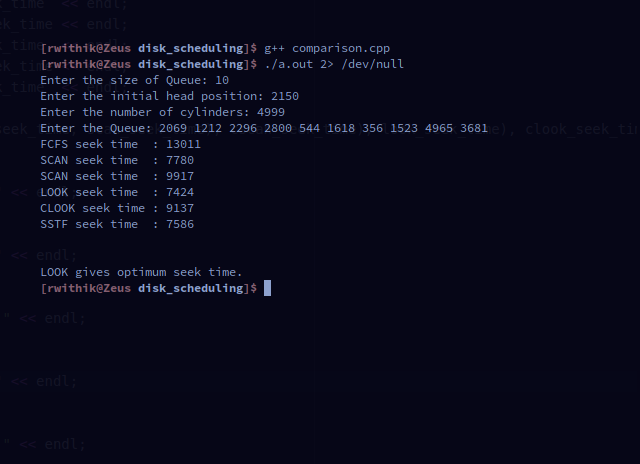
\includegraphics[width=\linewidth]{../Images/disk_scheduling/comparison.png}\newline

\section*{Header Files}

\subsection*{FCFS}

\inputminted{c++}{../Programs/disk_scheduling/fcfs.cpp}


\subsection*{SCAN}

\inputminted{c++}{../Programs/disk_scheduling/scan.cpp}


\subsection*{C-SCAN}

\inputminted{c++}{../Programs/disk_scheduling/cscan.cpp}


\subsection*{LOOK}

\inputminted{c++}{../Programs/disk_scheduling/look.cpp}


\subsection*{C-LOOK}

\inputminted{c++}{../Programs/disk_scheduling/clook.cpp}


}
\end{document}
